本章では,本手法の有効性を記すための評価実験について示す.

\section{実験概要}
SSDにより検出された変形ARマーカの姿勢推定を仮定して,評価を行う.
提案手法をバッチサイズ100,エポック数500で学習を行い変形ARマーカID0~9を平面への復元を行い
ID0の変形ARマーカを使用して姿勢推定を行う.
学習データ,データベース,推論データは,第2章で作成したものを使用する.
姿勢推定で用いる推論データは姿勢が分かるように姿勢情報を保存したものを用いる.
半径20,30,40mmの円柱それぞれ
100枚の背景テクスチャ付き変形ARマーカをランダム姿勢
で撮影した画像を使用する.
それぞれの推論結果は平均絶対誤差(MAE)を用いて推定された姿勢と正解姿勢の誤差を求める.
推論結果の平均のroll,pitch,yaw,平均誤差の4項目を求めて確認する.
MAEとは平均絶対2乗誤差の事であり2つのデータの誤差を絶対値で求め平均を取る誤差の指標である.
この実験で本手法による変形ARマーカの姿勢推定の精度を確認する.
なお,ここでの姿勢の角度は度数法によって表現する.

\newpage

\section{実験環境}
実験環境を表\ref{tab:kankyo}に示す.

\begin{table}[h]
  \centering
  \caption{実験環境}
    \begin{tabular}{c||c} \hline
    	OS & Ubuntu16.04 LTS \\ \hline
    	CPU &  Intel® Core™ i7-8700K CPU @ 3.70GHz × 12 \\ \hline
    	GPU & GeForce GTX 1080/PCle/SSE2 \\ \hline
     メモリ & 15.6 GiB \\ \hline
    	Python & 3.5.2 \\ \hline
    	Pytorch & 1.3.1 \\ \hline
  \end{tabular}
 \label{tab:kankyo}
\end{table}


\section{実験結果}

\subsection{提案手法による復元結果}
それぞれのID に対して,左から正解画像,変形ARマーカ画像,復元画像である.

\begin{itemize}
\item ID0
\end{itemize}

ID0の復元画像の出力結果を図\ref{i0}に示す.

      \begin{figure}[htbp]
      \begin{center}
      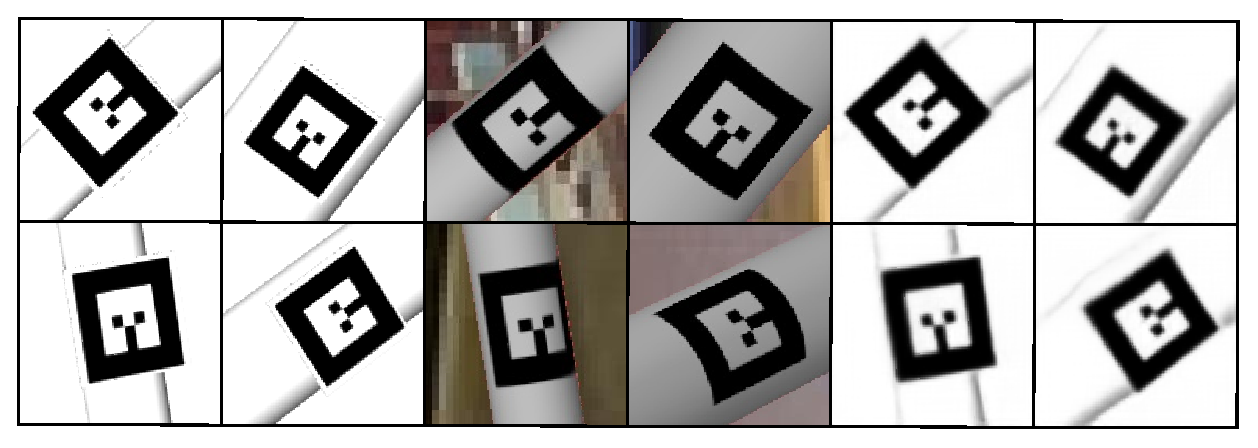
\includegraphics[width=85mm]{figure/eps/F0.eps}
      \caption{ID0の復元結果.}
      \label{i0}
      \end{center}
      \end{figure}
\newpage

\begin{itemize}
\item  ID1
\end{itemize}

ID1の復元画像の出力結果を図\ref{i1}に示す.

      \begin{figure}[htbp]
      \begin{center}
      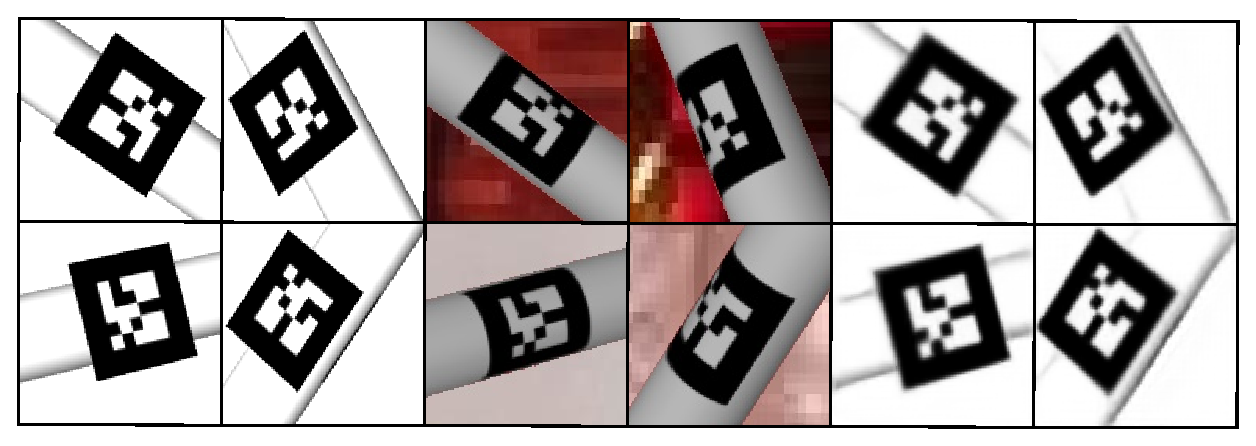
\includegraphics[width=85mm]{figure/eps/F1.eps}
      \caption{ID1の復元結果.}
      \label{i1}
      \end{center}
      \end{figure}


\begin{itemize}
\item  ID2
\end{itemize}

ID2の復元画像の出力結果を図\ref{i2}に示す.

      \begin{figure}[htbp]
      \begin{center}
      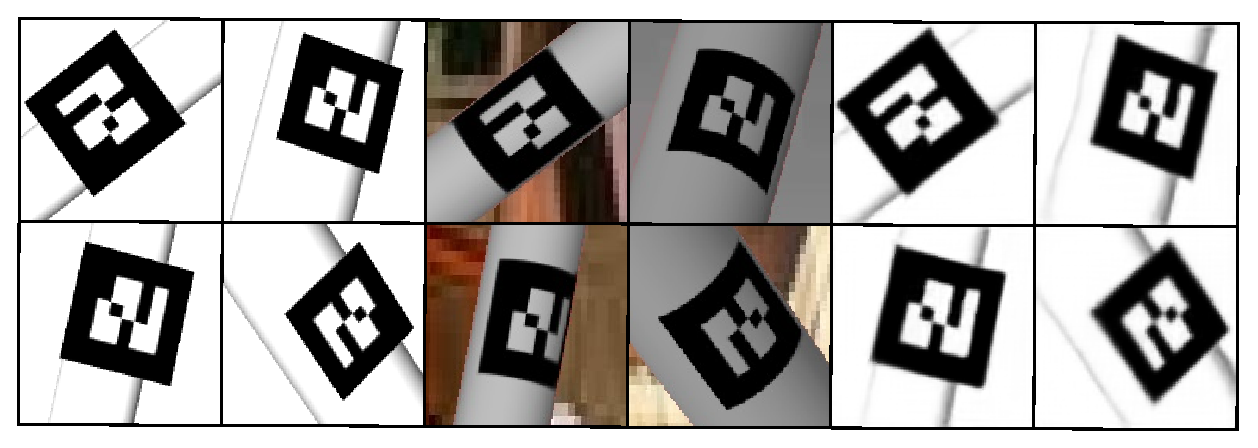
\includegraphics[width=85mm]{figure/eps/F2.eps}
      \caption{ID2の復元結果.}
      \label{i2}
      \end{center}
      \end{figure}


\begin{itemize}
\item  ID3
\end{itemize}

ID3の復元画像の出力結果を図\ref{i3}に示す.

      \begin{figure}[htbp]
      \begin{center}
      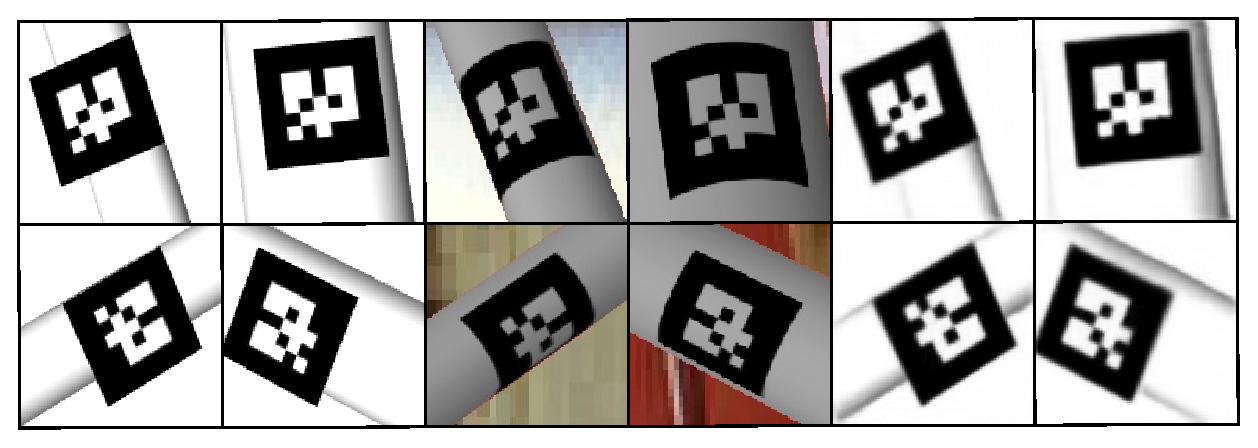
\includegraphics[width=85mm]{figure/eps/F4.eps}
      \caption{ID3の復元結果.}
      \label{i3}
      \end{center}
      \end{figure}

\newpage

\begin{itemize}
\item ID4
\end{itemize}

ID4の復元画像の出力結果を図\ref{i4}に示す.

      \begin{figure}[htbp]
      \begin{center}
      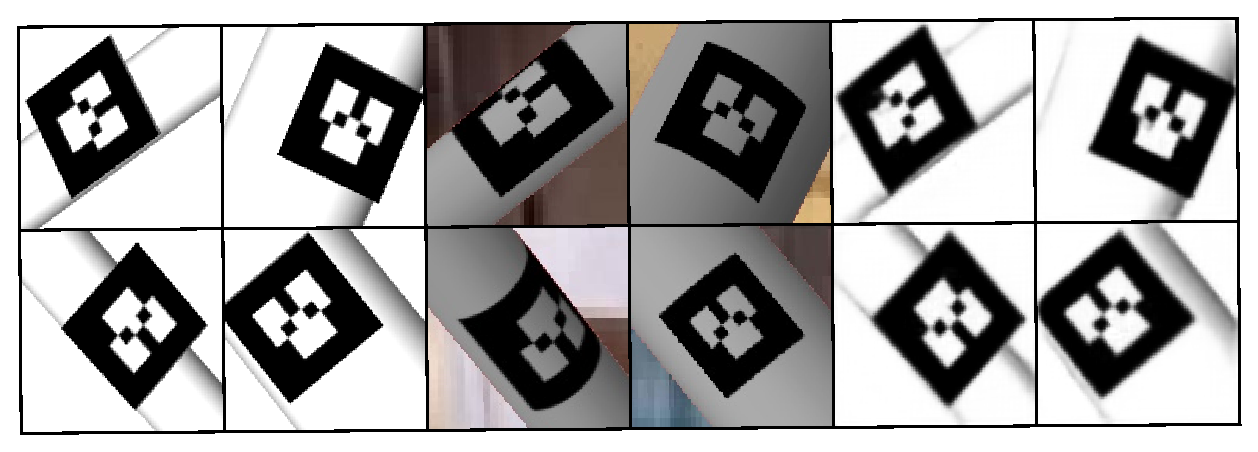
\includegraphics[width=85mm]{figure/eps/F5.eps}
      \caption{ID4の復元結果.}
      \label{i4}
      \end{center}
      \end{figure}


\begin{itemize}
\item  ID5
\end{itemize}

ID5の復元画像の出力結果を図\ref{i5}に示す.

      \begin{figure}[htbp]
      \begin{center}
      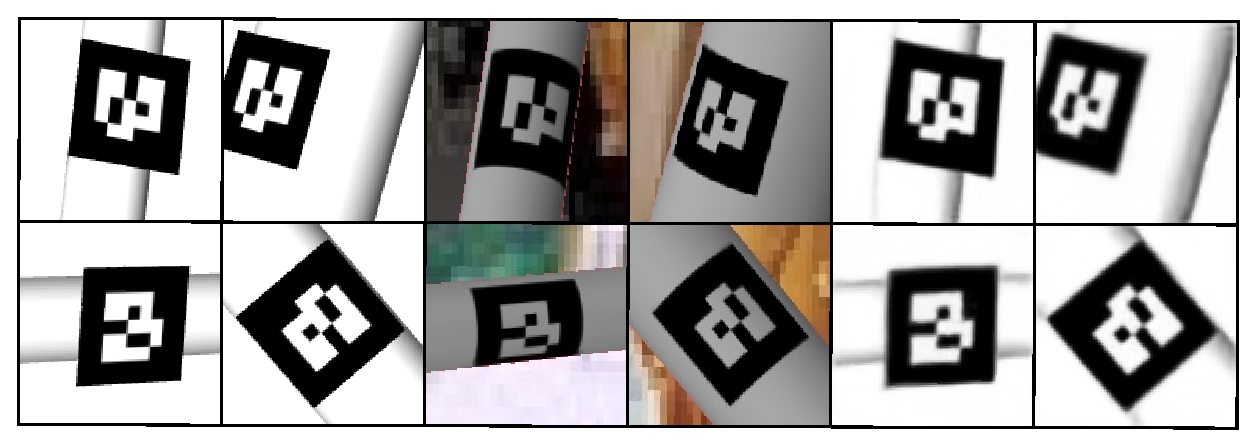
\includegraphics[width=85mm]{figure/eps/F6.eps}
      \caption{ID5の復元結果.}
      \label{i5}
      \end{center}
      \end{figure}



\begin{itemize}
\item  ID6
\end{itemize}

ID6の復元画像の出力結果を図\ref{i6}に示す.

      \begin{figure}[htbp]
      \begin{center}
      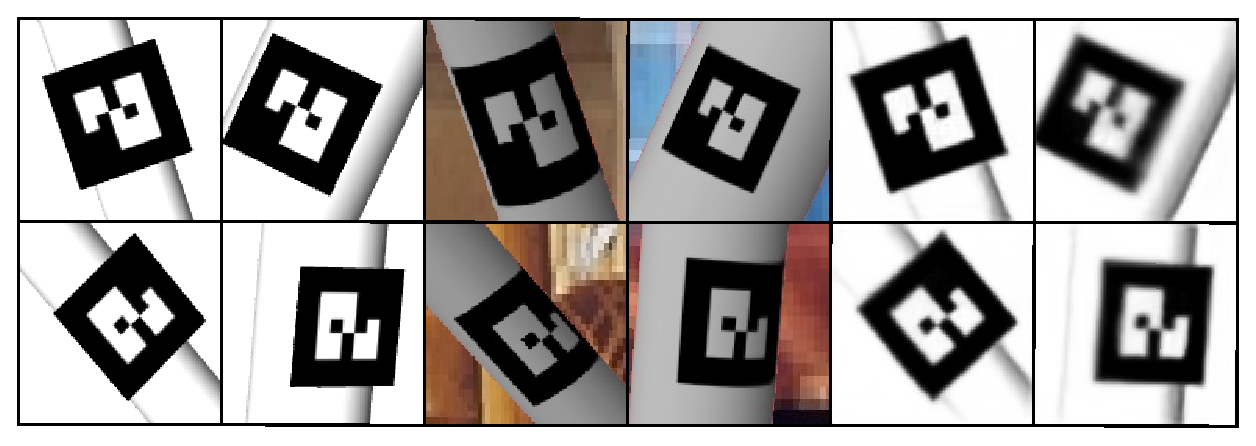
\includegraphics[width=85mm]{figure/eps/F7.eps}
      \caption{ID6の復元結果.}
      \label{i6}
      \end{center}
      \end{figure}

\newpage
\begin{itemize}
\item  ID7
\end{itemize}

ID7の復元画像の出力結果を図\ref{i7}に示す.

      \begin{figure}[htbp]
      \begin{center}
      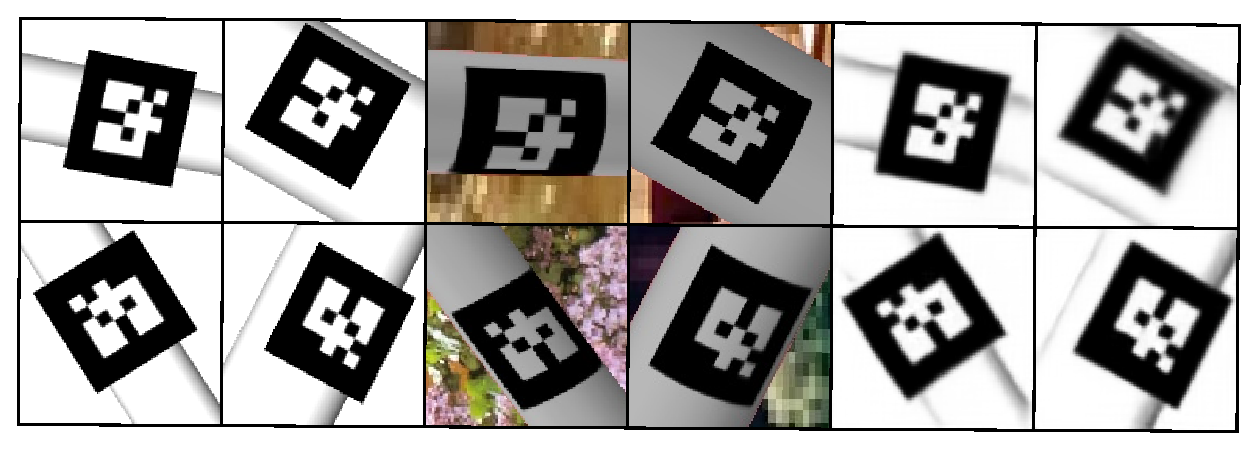
\includegraphics[width=85mm]{figure/eps/F8.eps}
      \caption{ID7の復元結果.}
      \label{i7}
      \end{center}
      \end{figure}



\begin{itemize}
\item  ID8
\end{itemize}

ID8の復元画像の出力結果を図\ref{i8}に示す.

      \begin{figure}[htbp]
      \begin{center}
      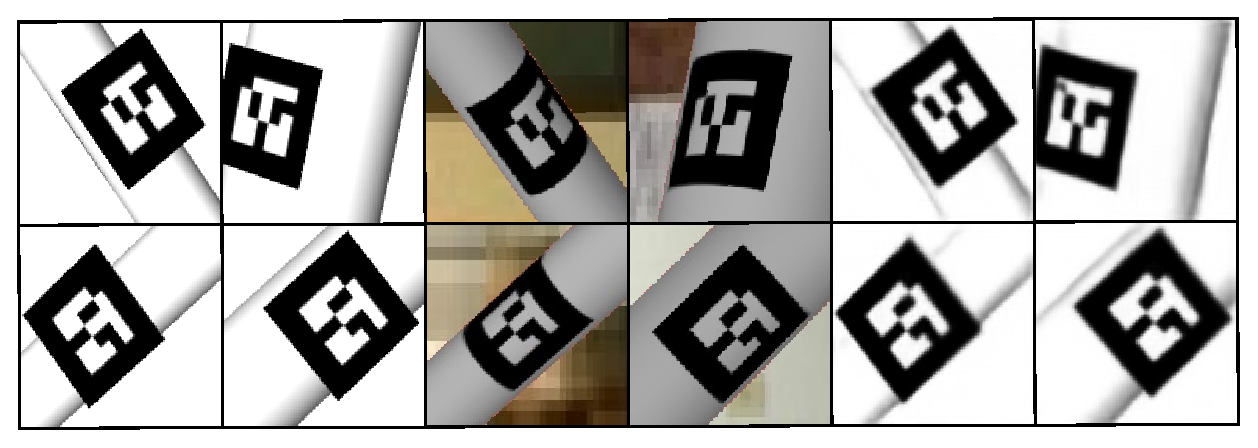
\includegraphics[width=85mm]{figure/eps/F9.eps}
      \caption{ID8の復元結果.}
      \label{i8}
      \end{center}
      \end{figure}


\begin{itemize}
\item  ID9
\end{itemize}

ID9の復元画像の出力結果を図\ref{i9}に示す.

      \begin{figure}[htbp]
      \begin{center}
      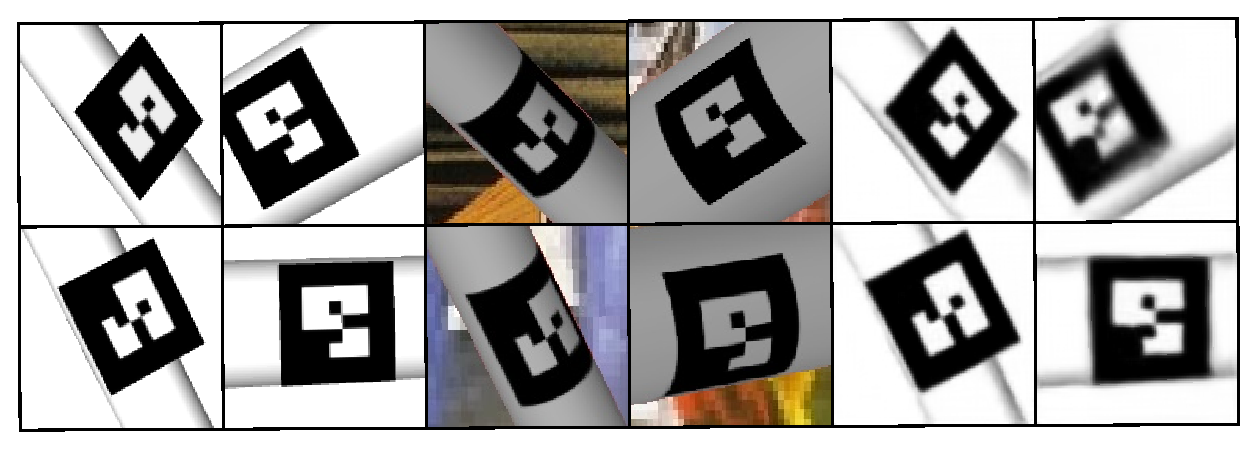
\includegraphics[width=85mm]{figure/eps/F10.eps}
      \caption{ID9の復元結果.}
      \label{i9}
      \end{center}
      \end{figure}


\subsection{提案手法を用いた姿勢推定結果}
提案手法により推定された各円柱半径における推論データ100枚の
roll,pitch,yaw,姿勢全体におけるMAEを表\ref{hyouka}に示す.



\begin{table}[h]
        \vspace{0zh}
          \begin{center}
            \caption{提案手法における姿勢推定の精度}
            \label{hyouka}
            \begin{tabular}{c|c|c|c|c} \hline
              円柱半径[mm]   & roll& pitch & yaw&姿勢全体 \\ \hline
              20& 5.30 & 3.64 & 3.42&4.12 \\ \hline
              30&5.78 & 4.49 & 3.71& 4.66 \\ \hline
              40&6.52 &4.51  &3.71&4.91 \\ \hline
              \end{tabular}
          \end{center}
        \vspace{-1.0zh}
\end{table}





\section{考察}
表\ref{hyouka}より,姿勢推定誤差のMAEは平均4~5前後の誤差という結果となり,半径の小さいARマーカほど推定結果がよくなっている.これは円柱の半径が小さいほど姿勢ごとに画像の特徴量が大きく変わるため,潜在変数が明確になるという事がこの結果の要因である.また,データベースの分解能を3度で用意したことにより,類似度計算を行う際にまったく同じ姿勢データがあると限らなかった.その為,推定誤差が生じるという結果になった.データベースの分解能を1度に設定し用意しておくことで範囲内の姿勢であればすべての角度に対応出来るため推定精度が上がると考えられる.

復元結果で示したように,提案手法による復元は行えているが,明確に表現されていない部分もある.今回は学習画像を1種類あたり1500枚で行ったが,学習画像のバリエーションを増やすことで変形ARマーカの潜在変数をより明確に取得することが可能となる.その為学習のバリエーションを増やすことで,復元精度・推定精度はともに高くなると考えられる.
















